% vim: foldmethod=marker: 
\documentclass[11pt,a4paper]{article}

%|--- Packages and Configs {{{1
\usepackage[utf8]{inputenc}
\usepackage[T1]{fontenc}    
%\usepackage[brazil]{babel}

\usepackage{xcolor}

\usepackage{amsmath}
\usepackage{amsfonts}
\usepackage{amssymb}
\usepackage{amsthm}
\usepackage{mathrsfs}

%\usepackage[top=2cm, bottom=2cm, left=2cm, right=2cm]{geometry}
\usepackage{mathtools}
\usepackage{hyperref}
\usepackage{enumerate}

%\usepackage{bbm} %% \mathbbm{1} gives you the identity function symbol 1

%%% allows you to insert many figures indexed by (a), (b), ... on a figure environment
\usepackage{float} 
\usepackage[caption = false]{subfig}

\usepackage{tikz}

\usepackage{ifthen} %% gives if conditionals when using newcommand

%\setcounter{secnumdepth}{0} %%% this will print the section titles on tableofcontens without inserting numbers.
%% Garamond fonts 
%% \usepackage{ebgaramond}
%% \usepackage[ugm]{mathdesign}
% 1}}}

%|--- Author, Title and Date {{{1
\title{Documentation of the C code used to calculate the path persistent homology (aka pph)
       up to diagrams of dimension 0 and 1}
\author{Rafael Polli Carneiro}
\date{} 
% 1}}}

%|--- Math operators {{{1
\DeclareMathOperator{\Z}{\mathbb{Z}}
\DeclareMathOperator{\R}{\mathbb{R}}
\DeclareMathOperator{\allowtime}{allow time}
\DeclareMathOperator{\entrytime}{entry time}
\DeclareMathOperator{\definedAs}{\vcentcolon = }
%\DeclareMathOperator {\card}{card}
%\DeclareMathOperator {\Id}{\mathbbm{1}}
%
%
%
%\DeclareTextFontCommand{\emph}{\bfseries\em} %% redefining \emph{} with bold and italic font
%
%\DeclareMathOperator {\Imagem}{ Im }
% 1}}}

%|--- Begin Document {{{1
\begin{document}
\maketitle
\tableofcontents

%|--- Initiall Observations {{{2
\section{Initiall Observations}
Be warned that henceforth we will admit the following conventions:
\begin{enumerate}[i)]
	\item Whenever talking about vector spaces, namelly $V$, we have that the field acting
		onto $V$ is going to be $\Z_2$;

	\item Every vector space here has finite dimension;
\end{enumerate}
% END Initiall Observations 2}}}

%|--- How It is structured {{{2
\section{How The Program is structured}
Everything here, concerning the \texttt{C} code, is splitted into the two folders: \textit{headers}, \textit{src}.
Inside headers one can find the data types which are used to perform the main algorithm, as well
the respectivelly functions prototypes that operate with these data types. Finaly, \textit{src} is merely the
\texttt{C} implementation of such functions.
%, or methods if someone prefers to call them.
%The \texttt{C} code called \textit{main.c}, runs the algorithm desired to be calculated.
% END How It is structured 2}}}

%|--- Headers {{{2
\section{Headers}
The folder Headers has the following tree structure:
\begin{figure}[H]
	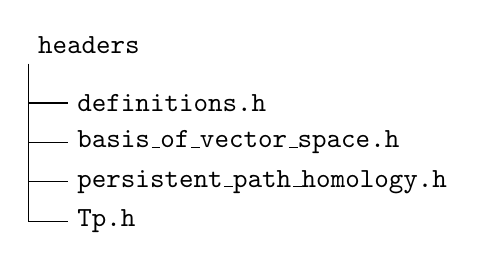
\begin{tikzpicture}[scale=0.5]
		\draw (0,0) node[anchor=south west] {\texttt{headers}};
		\draw (0,0) -- (0,-1) -- (1, -1) node[anchor=west] {\texttt{definitions.h}};
		\draw (0,-1) -- (0,-2) -- (1, -2) node[anchor=west] {\texttt{basis\_of\_vector\_space.h}};
		\draw (0,-2) -- (0,-3) -- (1, -3) node[anchor=west] {\texttt{persistent\_path\_homology.h}};
		\draw (0,-3) -- (0,-4) -- (1, -4) node[anchor=west] {\texttt{Tp.h}};
	\end{tikzpicture}
	\caption{tree headers.}
\end{figure}

Now let's describe each file contained at \texttt{headers}.

%|--- definitions.h {{{3
\subsection{\textit{definitions.h}}
Here, basic, yet fundamental data types are defined. To begin with, 
we have the following constants:
\begin{itemize}
	\item  \texttt{TRUE} or \texttt{FALSE};

	\item  \texttt{MARKED} or \texttt{NOT\_MARKED}. Here, these flags address whether or not
		an element of a vector space, more precisely, an element of its basis, is marked of not.

	\item \texttt{EMPTY} or \texttt{NOT\_EMPTY}. We say that the ith element of an array can be empty
		or not, meaning that nothing has been allocated at its memomery space, if it is
		empty, and the contrary otherwise;

	\item \texttt{SORTED} or \texttt{NOT\_SORTED}. ???;
\end{itemize}

%|--- data types {{{4
\subsubsection{Data types}
The data types are:
\begin{itemize}
	\item \texttt{boolean} = TRUE or FALSE;

	\item \texttt{vertex\_index} = $0, 1, 2, \ldots, N$. Given a graph $(G,V)$, each vertex (or node
		if you prefer to call it), will be enumerated by integers $\geq 0$;

	\item \texttt{base\_index}. Let $V$ be a vector space. Then, considering $\beta \subseteq V$
		as its base, with $\beta = \{v_0, v_1, \ldots, v_N\}$, we say that
		$0, 1, 2, \ldots$ will be elements of the \texttt{base\_index};

	\item \texttt{vector\_index}. Given a enumeration of vectors, \texttt{vector\_index} stores
		the indexes of such enumeration. For instance, let the vectors $v_0, v_1, v_2, \ldots$.
		Then the indexes $0,1,2,\ldots$ are elements of \texttt{vector\_index}.
%	\item \texttt{vector\_index}. Any element of a vector space $V$, i.e., a vector, can be written
%		as coordinates, given a fixed basis. Thus, let's say that $V \ni u = (0, 1, 1, 0, 1)$.
%		Then the non-negative integers $0, 1, 2, 3, 4$ are elements of the data type 
%		\texttt{vector\_index}, with $u_0 = 0, u_1 = 1, u_2 = 1, u_3 = 0, u_4 = 1$;

	\item \texttt{dim\_path}. Let $(G,A)$ be a graph. Then $w = [a_0, a_1, \ldots, a_N]$
		is called a regular path in $G$ if $\forall i \in \{0, 1, \ldots, N\}$ the following holds
		\[
			a_i \in G \quad \text{and} \quad (a_0, a_1), (a1, a_2), \ldots, (a_{N-1}, a_{N}) 
			\text{are edges of the graph}.
		\]
		The regular path $w$, in this case, is said to have dimension $N$. Consequently, \texttt{dim\_path}
		will be the data type responsible of representing all dimension of possible regular paths
		being used in the future;

	\item \texttt{dim\_vector\_space}. The meaning of this data type can be understood immeadiately;

	\item \texttt{regular\_path}. A regular path is exactly what was described up abpve,
		that is, $w = [a_0, a_1, \ldots, a_N]$ is a regular path when each $a_i$ is a node, forall $i$,
		and every pair $(a_0,a_1), (a_1, a_2), \ldots, (a_{N-1}, a_N)$ is an edge. It is natural to represent
		a regular path as an array and, in fact, that is the way they will be represented in
		here. Thus, the type 
		\texttt{regular\_path} is, as expected, a pointer to \texttt{vertex\_index} types.
		See Figure~\ref{fig:regular_path} for a visual explanation.
		\begin{figure}
			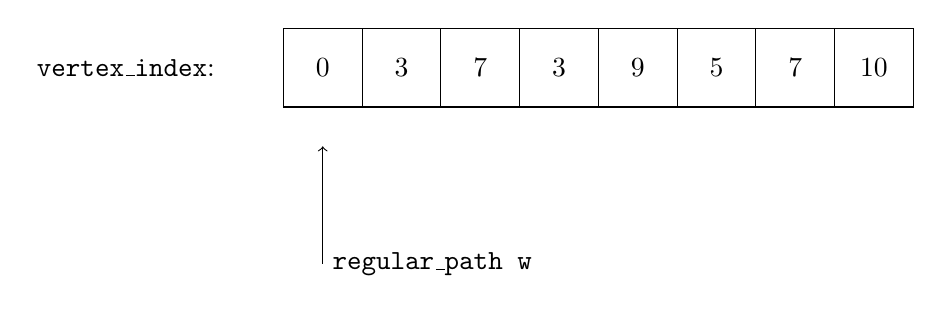
\begin{tikzpicture}
				\def \y {0.5}
				\def \xx {1.5}

				\draw (-1,\y) node {\texttt{vertex\_index}:};
				\foreach \x\z in {1/0,2/3,3/7,4/3/,5/9,6/5,7/7,8/10} {
					\draw (\x,0) rectangle (\x+1,1) node [midway] {$\z$};
				}
				\draw[<-] (\xx,-0.5) -- (\xx, -2.0) node[anchor=west] {\texttt{regular\_path w}};
			\end{tikzpicture}
			\caption{Representation of a regular path $w = [0,3,7,3,9,5,7,10]$.}
			\label{fig:regular_path}
		\end{figure}

	\item \texttt{vector}. Considering $V$ a vector space with basis $\beta \subseteq V$, then
		any element of $V$ can be seen as its coordinates. For instance,
		let $w = (0,0,0,0,1,1,0) \in V$. The data type \texttt{vector}
		is, as \texttt{regular\_path}, a pointer to \texttt{boolean},
		which are elements of $\Z_2$. 
		{\color{red} For large graphs, and due to the fact that the array
		vector is filled with many zeros (in my analysis), this data type is
		not the best to be used. I WILL CHANGE IT FOR  A LIST!!!}
\end{itemize}
%END data types 4}}}

%|--- functions {{{4
\subsubsection{Functions}
Finnaly, the following functions, down below, will implement some routines over the data types
defined into \texttt{definitions.h}. They are:
\begin{description}
	\item [\textit{are\_these\_regular\_paths\_the\_same}] \hfill \\[-0.5cm]
		\begin{description}
			\item [Parameters]: \texttt{regular\_path},\texttt{regular\_path}, \texttt{dim\_path}.
			\item [Objective]: Check if two regular paths $w_1, w_2$ are equal.
				In case positive it returns TRUE, and FALSE otherwise.
			\item [Return]: \texttt{boolean}.
		\end{description}

	\item [\texttt{is\_this\_path\_a\_regular\_path}] \hfill \\[-0.5cm]
		\begin{description}
			\item [Parameters]: \texttt{regular\_path}, \texttt{dim\_path}.
			\item [Objective]: It checks if an the array $w = [a_0, a_1, \ldots, a_N]$
				is a regular path, that is, the pairs $(a_0, a_1), (a_1,a_2),
				\ldots, (a_{N-1}, a_N)$ are, indeed, edges of the graph.
				This function is important specially when taking a border
				operator of a regular path which, in most cases, the outcome
				can incorporate non regular paths. It returns TRUE if $w$
				is a regular path, and FALSE otherwise.
			\item [Return]: \texttt{boolean}.
		\end{description}

	\item [\texttt{is\_this\_vector\_zero}] \hfill \\[-0.5cm]
		\begin{description}
			\item [Parameters]: \texttt{vector}, \texttt{dim\_vector\_space}.
			\item [Objective]: It checks if a vector $v$ of a vector space is
				zero, returning TRUE if positive and FALSE otherwise
			\item [Return]: \texttt{boolean}.
		\end{description}

	\item [\texttt{sum\_these\_vectors}] \hfill \\[-0.5cm]
		\begin{description}
			\item [Parameters]: \texttt{vector}, \texttt{vector}, \texttt{dim\_vector\_space}.
			\item [Objective]: Let $w_1, w_2$ two elements of a vector space.
				Then this function returns a vector with the value equal
				to the sum $w_1 + w_2$.
			\item [Return]: \texttt{vector}.
		\end{description}
\end{description}
% END Functions 4}}}
% END definitions 3}}}

%|--- basis_of_vector_space.h {{{3
\subsection{basis\_of\_vector\_space.h}

This header will provide us an abstraction of  vector spaces which are spanned by a collection of regular paths.
Bare in mind that in our context we have a sequence of sets of regular paths, indexed by $i \in \R_{\geq 0}$,
given by
\[
	R^p_i = \{ [a_0, a_1, \ldots, a_p]; f(a_0, a_1) \leq i, f(a_1, a_2) \leq i, \ldots, f(a_{p-1}, a_p) \},
\]
where $a_0, a_1, \ldots, a_p$ nodes of a graph and $f:G \times G \to \R_{\geq 0}$ a matrix. This provide
a sequence 
\[
	\R_i \subseteq \R_{j}, 
\]
whenever $0 \leq i \leq j$. This is called a filtration, and it will provide us times which
homological features appears and dissapear. With that in mind, for every regular path 
$w = [a_0, a_1, \ldots, a_p$,
we define
\[
	\allowtime(w) \definedAs \inf \{ i \in \R_{\geq 0}; f(a_0, a_1) \leq i, f(a_1, a_2) \leq i,
	\ldots, f(a_{p-1}, a_p) \}
\]
and 
\[
	\entrytime(w) \definedAs \min\{\allowtime(w), \allowtime(\partial(w))\};
\]
with $f$ that matrix associated with the graph and $\partial$ the border operator.

%|--- Data types {{{4
\subsubsection{Data Types}
With these operators in mind we start by the following data types:
\begin{itemize}
	\item \texttt{tuple\_regular\_path\_double}. Given a base $\beta$ of regular paths, then
		\texttt{tuple\_regular\_path\_double} is a structure composed
		by the ith regular path of the base $\beta$ and by the 
		allow time of such regular path.
		See Figure~\ref{fig:data_type_basis_of_vs}.

	\item \texttt{base}. This is a structure that will be responsible to store all
		elements of a base which are regular paths of same
		dimension. Thus \texttt{base\_matrix} is a pointer to 
		\texttt{tuple\_regular\_path\_double} where the regular paths must 
		have the dimendion given by \texttt{dimension\_of\_the\_regular\_path}.\\
		The dimension of the vector space spaned by the base \texttt{base\_matrix}
		is stored at \texttt{dimension\_of\_the\_vs\_spanned\_by\_base}.
		Finally, \texttt{marks} is an array of
		the same size of \texttt{base\_matrix} where it shows if the ith element
		of the base is marked or not.
		See Figure~\ref{fig:data_type_basis_of_vs}. Notice that in the 
		Figure~\ref{fig:data_type_basis_of_vs}	only \texttt{base\_matrix} is
		represented, while the other features are left inside the center
		dots (this is done beacuse \texttt{base\_matrix} is the 
		object that should be paid more atention).

	\item \texttt{collection\_of\_basis}. This is a structure which can be seen as
		the union of every base indexed by the dimension of the paths
		that generates each vector space. Here \texttt{max\_of\_basis}
		counts how many basis do we have, taking into consideration that we start counting 
		from zero.
		See Figure~\ref{fig:data_type_basis_of_vs}.
\end{itemize}

%|--- fig:data_type_basis_of_vs {{{5
\begin{figure}[H]
	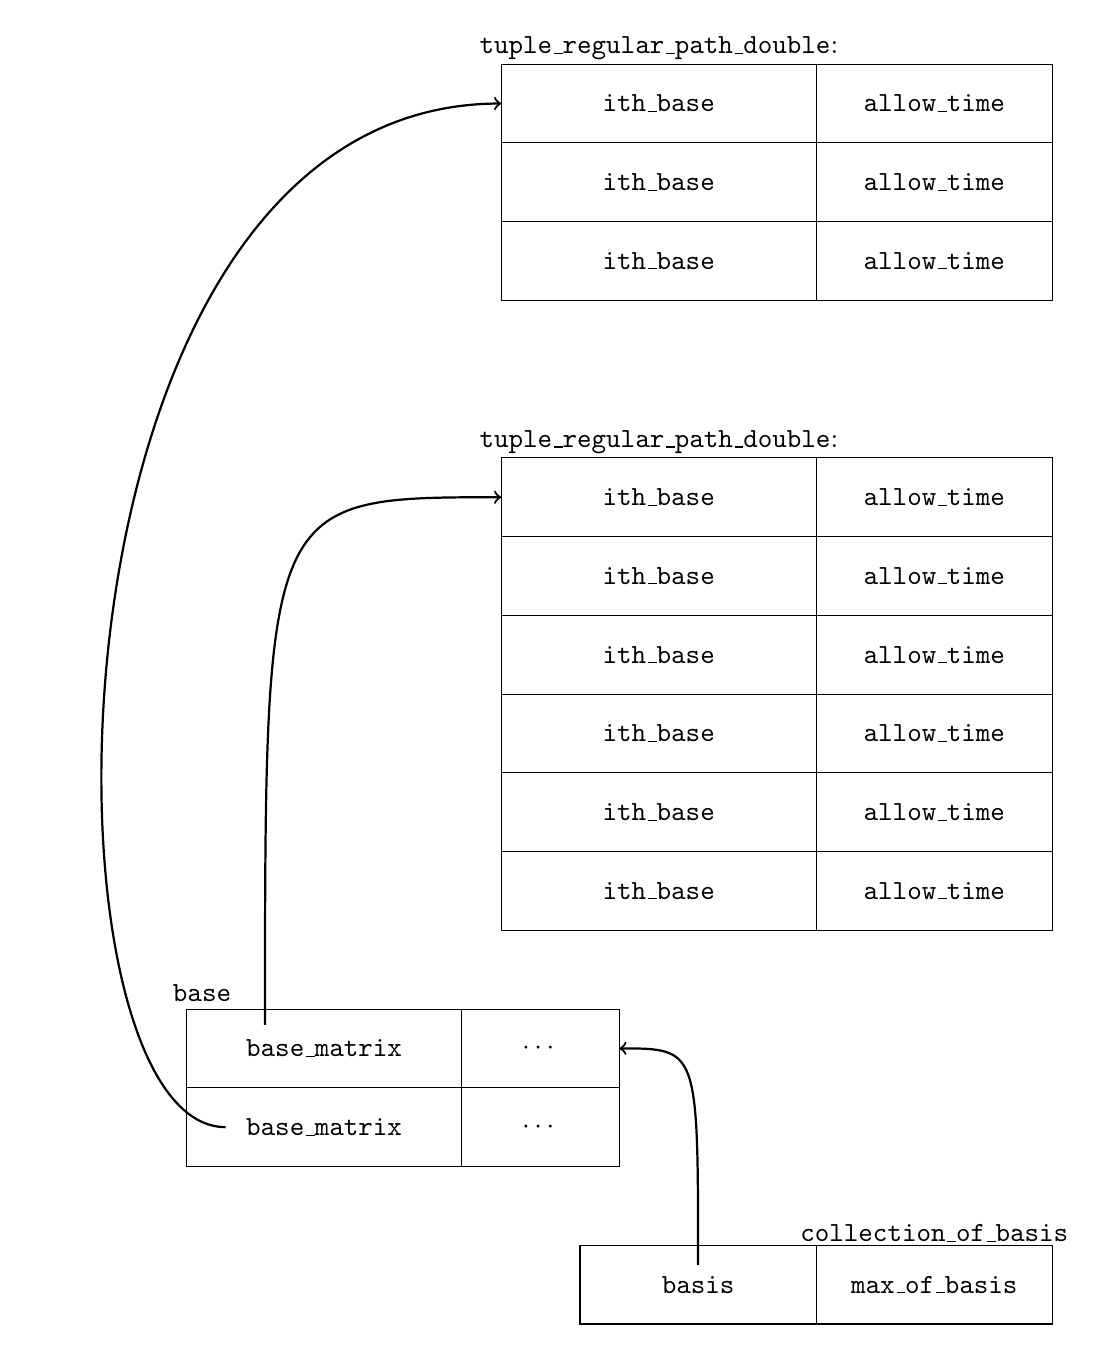
\begin{tikzpicture}
		\def \x {3}
		\def \xb {-1}

		\draw (2.6,6.2) node[anchor=west] {\texttt{tuple\_regular\_path\_double}:};
		\foreach \y in {0, 1, ..., 5} {
			\draw (\x,  \y) rectangle (\x+4,  \y+1) node[midway] {\texttt{ith\_base}};
			\draw (\x+4,\y) rectangle (\x+4+3,\y+1) node[midway] {\texttt{allow\_time}};
		}

		\draw (2.6,11.2) node[anchor=west] {\texttt{tuple\_regular\_path\_double}:};
		\foreach \y in {8,9,10} {
			\draw (\x,  \y) rectangle (\x+4,  \y+1) node[midway] {\texttt{ith\_base}};
			\draw (\x+4,\y) rectangle (\x+4+3,\y+1) node[midway] {\texttt{allow\_time}};
		}


		\draw (\xb+0.2,-0.8) node {\texttt{base}};
		\foreach \y in {0,1} {
			\draw (\xb,  -2-\y) rectangle (\xb+3.5,  -1-\y) node[midway] {\texttt{base\_matrix}};
			\draw (\xb+3.5,-2-\y) rectangle (\xb+2+3.5,-1-\y) node[midway] 
			{$\cdots$};
		}
		
		\draw[->, thick] (\xb+1, -1.2) .. controls (\xb+1, 5.5) and (\xb+1, 5.5) .. (\x, 5.5);
		\draw[->, thick] (\xb+0.5, -2.5) .. controls (\xb-2, -2.5) and (\xb-2, 10.5) .. (\x, 10.5);

		\draw (\x+1, -5) rectangle (\x+1+3,-4) node[midway] {\texttt{basis}};
		\draw (\x+1+3, -5) rectangle (\x+1+3+3,-4) node[midway] {\texttt{max\_of\_basis}};

		\draw[->,thick] (\x+2.5, -4.25) .. controls (\x+2.5,-1.5) and (\x+2.5,-1.5) .. (\xb+2+3.5, -1.5);
		\draw (\x+5.5, -3.85) node {\texttt{collection\_of\_basis}};
	\end{tikzpicture}
	\caption{Visual reresentation of the data types defined at the file
	\texttt{basis\_of\_vector\_space.h}.}
	\label{fig:data_type_basis_of_vs}
\end{figure}
% END fig:data_type_basis_of_vs 5}}}

% END Data Types 4}}}

%|--- Functions {{{4
\subsubsection{Functions}
We start with the two functions responsible for allocating all possible 
regular paths into their respectively basis:
\begin{description}
	\item [\textit{alloc\_all\_basis}] \hfill \\[-0.5cm]
		\begin{description}
			\item [Parameters]: \texttt{unsigned\_int}, \texttt{unsigned\_int}, \texttt{double**}.
			\item [Objective]: Given an integer $N$, this function will allocate
				$N+1$ basis, taking as reference the amount of nodes of 
				the graph and its network weight matrix.\\
				(Obs: the function
				\texttt{generating\_all\_regular\_paths\_dim\_p} is used)
				Also, regular paths of dimension 0 are stored by this function.
			\item [Return]: \texttt{collection\_of\_basis*}.
		\end{description}

	\item [\textit{generating\_all\_regular\_paths\_dim\_p\_version2}] \hfill \\[-0.5cm]
		\begin{description}
			\item [Parameters]: \texttt{collection\_of\_basis*}, \texttt{double**}.
			\item [Objective]: Given a \texttt{collection\_of\_basis*} this function
				will all regular paths of dimension $1$ and $2$
				into the structures which represent the basis of the 
				vector spaces spanned by such regular paths.
				\textit{generating\_all\_regular\_paths\_dim\_p\_version2}
				will be used by the function above.
			\item [Return]: \texttt{void}.
		\end{description}
\end{description}

Now, in order to the main algorithm to work we need to be able to ``mark'' a vector
basis. The first thing that I do is to initialize arrays where their index are in correspondence
with the index of the \texttt{base\_matrix}. Then, a function is definined so, in the runtime,
it is possible to mark a given vector basis.
\begin{description}
	\item [\textit{initialize\_Marking\_basis\_vectors}] \hfill \\[-0.5cm]
		\begin{description}
			\item [Parameters]: \texttt{collection\_of\_basis}
			\item [Objective]: For each dimension of regular paths up to
				\texttt{max\_of\_basis}, an array, namely \texttt{marks},
				of size \texttt{dimension\_of\_the\_vs\_spanned\_by\_base}
				is created so we will be able to say if a vector basis
				is marked or not
			\item [Return]: void
		\end{description}
	\item [\textit{marking\_basis\_vectors}] \hfill \\[-0.5cm]
		\begin{description}
			\item [Parameters]: \texttt{collection\_of\_basis}, \texttt{dim\_path},
				\texttt{base\_index}
			\item [Objective]: Mark a vector of a basis where all regular paths
				have dimension equal to a \texttt{dim\_path}.
			\item [Return]: void
		\end{description}
\end{description}

When we have all basis of regular paths allocated in memory we need to sort each base
by the allow time of its elements. In other words, let $\beta = \{a_o, a_1, a_2, \ldots, a_p\}$
be the base of the vector space spanned by regular paths of dimension $N$. Then we need
to ensure that
\[
	\allowtime(a_0) \leq \allowtime(a_1) \leq \allowtime(a_2) \leq \cdots.
\]
This is done by the function
\begin{description}
	\item [\textit{sorting\_the\_basis\_by\_their\_allow\_times}] \hfill \\[-0.5cm]
		\begin{description}
			\item [Parameters]: \texttt{collection\_of\_basis}
			\item [Objective]: Sort each element of a \texttt{base\_matrix} by
				the allow time of each \texttt{tuple\_regular\_path\_double}.
			\item [Return]: void
		\end{description}
\end{description}
which uses the function:
\begin{description}
	\item [\textit{compareTuple}] \hfill \\[-0.5cm]
		\begin{description}
			\item [Parameters]: \texttt{tuple\_regular\_path\_double},
				\texttt{tuple\_regular\_path\_double}
			\item [Objective]: This function induces a partial order into the space of
				regular paths by compairing allow times.
			\item [Return]: \texttt{int}
		\end{description}
\end{description}
to induce a partial order in the space of regular paths of same dimension.

Another important function is the one resposible to calculate the allow time of any
regular:
\begin{description}
	\item [\textit{allow\_time\_regular\_path}] \hfill \\[-0.5cm]
		\begin{description}
			\item [Parameters]: \texttt{network\_weight**},
				\texttt{regular\_path}, \texttt{dim\_path}
			\item [Objective]: It calculates the allow time of a \texttt{regular\_path} with
				dimension \texttt{dim\_path}.
			\item [Return]: \texttt{double}
		\end{description}
\end{description}

Last but not least, the getters and setters! Their meaning are straightforward.
\begin{description}
	\item [\textit{get\_dimVS\_of\_ith\_base}] \hfill \\[-0.5cm]
		\begin{description}
			\item [Parameters]: \texttt{collection\_of\_basis**}, \texttt{dim\_path}
			\item [Objective]: It returns the dimension of the vector space
				spanned by regular paths of dimension \texttt{dim\_path}
			\item [Return]: \texttt{dim\_vector\_space}
		\end{description}
	\item [\textit{set\_dim\_path\_of\_ith\_base}] \hfill \\[-0.5cm]
		\begin{description}
			\item [Parameters]: \texttt{collection\_of\_basis**}, \texttt{dim\_path}
			\item [Objective]: It sets the dimension of the regular paths that are going
				to be used
			\item [Return]: \texttt{void}
		\end{description}
	\item [\textit{set\_dimVS\_of\_ith\_base}] \hfill \\[-0.5cm]
		\begin{description}
			\item [Parameters]: \texttt{collection\_of\_basis**}, \texttt{dim\_path},
				\texttt{dim\_vector\_space}
			\item [Objective]: It sets the dimension of the vector space
				spanned by regular paths of dimension \texttt{dim\_path} to the
				values of \texttt{dim\_vector\_space}
			\item [Return]: \texttt{void}
		\end{description}
	\item [\textit{get\_path\_of\_base\_i\_index\_j}] \hfill \\[-0.5cm]
		\begin{description}
			\item [Parameters]: \texttt{collection\_of\_basis**}, \texttt{dim\_path},
				\texttt{base\_index}
			\item [Objective]: It returns a regular path of dimension 
				\texttt{dim\_path} which has the index of \texttt{base\_index}
			\item [Return]: \texttt{regular\_path}
		\end{description}
	\item [\textit{is\_path\_of\_dimPath\_p\_index\_j\_marked}] \hfill \\[-0.5cm]
		\begin{description}
			\item [Parameters]: \texttt{collection\_of\_basis**}, \texttt{dim\_path},
				\texttt{base\_index}
			\item [Objective]: It returns true if a regular path of dimension 
				\texttt{dim\_path} is marked and false otherwise 
			\item [Return]: \texttt{boolean}
		\end{description}
\end{description}
% END functions 4}}}

% END basis_of_vector_space.h 3}}}

%|--- Tp.h {{{3
\subsection{\texttt{Tp.h}}
Here we have the main structure responsible to take care with the 
gaussian elimination.

%|--- Data types {{{4
\subsubsection{Data Types}
The data types in here are going to be something equal to the ones found
to allocate the basis above.
\begin{itemize}
	\item \texttt{T\_p\_tuple}. A structure rpresenting a tuple $(v,e,m)$
		where $v$ is a \texttt{vector} whose coordinates represent
		the regular paths that decomposes $v$. Also, $e$
		is the \texttt{double} storing an entry time
		and $m$ is a \texttt{boolean} which informs
		if this tuple is empty or not.

	\item \texttt{T\_p\_tuple\_collection}. A collection of \texttt{T\_p\_tuple} which
		are indexed by a base of regular paths of the same dimension
		that spans a vector space of dimension \texttt{size}

	\item \texttt{T\_p}. A collection of all \texttt{T\_p\_tuple\_collection} up to \texttt{max\_of\_Tp},
		which will be equal to $1$.
\end{itemize}
Check Figure~\ref{fig:Tp} to understand these data types and notice that 
they follow the same pattern of the Figure~\ref{fig:data_type_basis_of_vs}.
%|--- fig:Tp {{{5
\begin{figure}[H]
	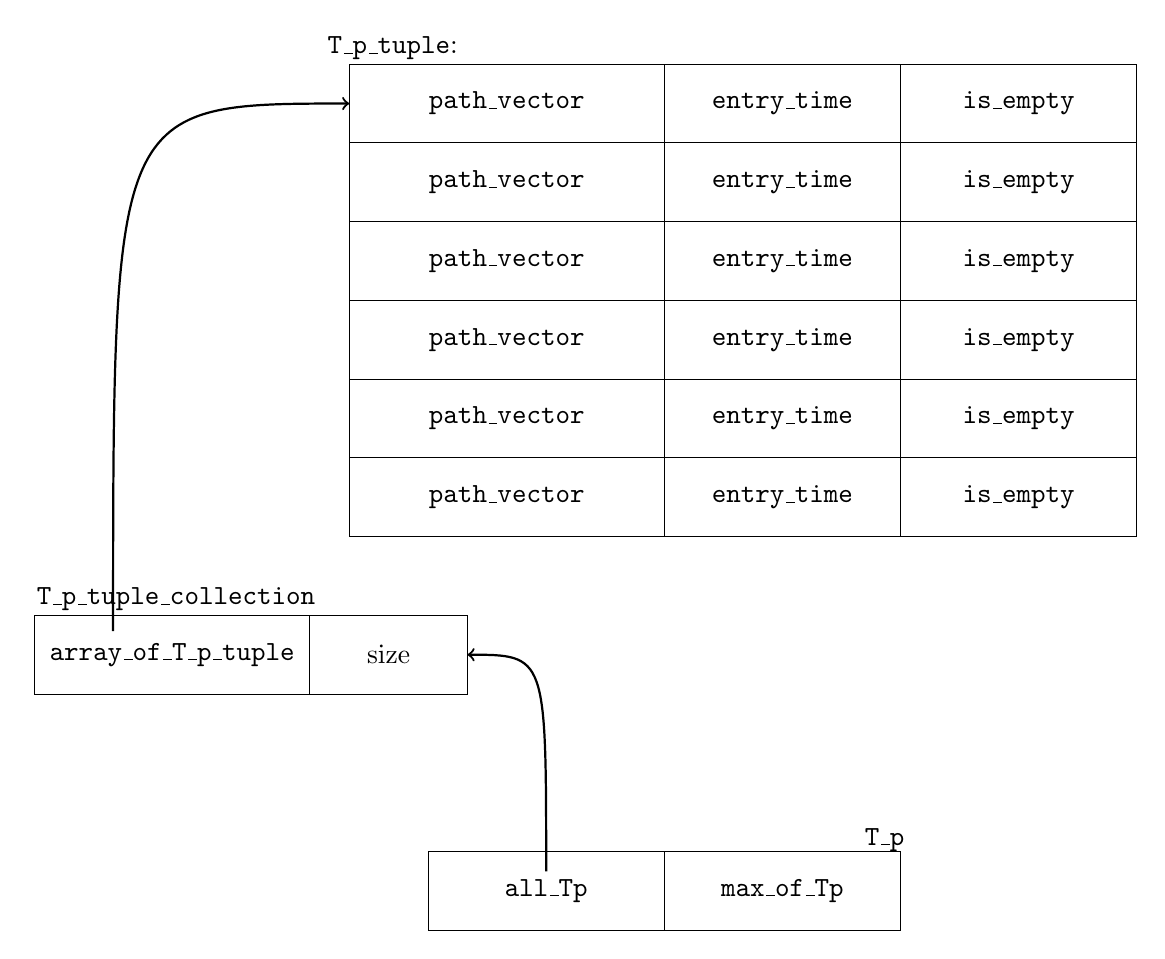
\begin{tikzpicture}
		\def \x {3}
		\def \xb {-1}

		\draw (2.6,6.2) node[anchor=west] {\texttt{T\_p\_tuple}:};
		\foreach \y in {0, 1, ..., 5} {
			\draw (\x,  \y) rectangle (\x+4,  \y+1) node[midway] {\texttt{path\_vector}};
			\draw (\x+4,\y) rectangle (\x+4+3,\y+1) node[midway] {\texttt{entry\_time}};
			\draw (\x+4+3,\y) rectangle (\x+4+3+3,\y+1) node[midway] {\texttt{is\_empty}};
		}

		\draw (\xb+1.8,-0.8) node {\texttt{T\_p\_tuple\_collection}};
		\foreach \y in {0} {
			\draw (\xb,  -2-\y) rectangle (\xb+3.5,  -1-\y) node[midway] {\texttt{array\_of\_T\_p\_tuple}};
			\draw (\xb+3.5,-2-\y) rectangle (\xb+2+3.5,-1-\y) node[midway] {size};
		}
		
		\draw[->, thick] (\xb+1, -1.2) .. controls (\xb+1, 5.5) and (\xb+1, 5.5) .. (\x, 5.5);

		\draw (\x+1, -5) rectangle (\x+1+3,-4) node[midway] {\texttt{all\_Tp}};
		\draw (\x+1+3, -5) rectangle (\x+1+3+3,-4) node[midway] {\texttt{max\_of\_Tp}};

		\draw[->,thick] (\x+2.5, -4.25) .. controls (\x+2.5,-1.5) and (\x+2.5,-1.5) .. (\xb+2+3.5, -1.5);
		\draw (\x+6.8, -3.85) node {\texttt{T\_p}};
	\end{tikzpicture}
	\caption{Visual reresentation of the data types defined at the file \texttt{Tp.h}.}
	\label{fig:Tp}
\end{figure}
% END fig:Tp 5}}}
%|--- END Data types 4}}}

%|--- Functions {{{4
\subsubsection{Functions}
\begin{description}
	\item [\textit{alloc\_T\_p}] \hfill \\[-0.5cm]
		\begin{description}
			\item [Parameters]: \texttt{collection\_of\_basis}.
			\item [Objective]: Function responsible to allocate all \texttt{T\_p} 
				structure into memory
			\item [Return]: \texttt{T\_p*}.
		\end{description}
\end{description}

Setters and getters.
\begin{description}
	\item [\textit{set\_T\_p\_pathdim\_i\_vector\_j}] \hfill \\[-0.5cm]
		\begin{description}
			\item [Parameters]: \texttt{T\_p*}, \texttt{dim\_path}, \texttt{vector\_index},
				\texttt{vector}, \texttt{double}.
			\item [Objective]: Allocate the \texttt{vector} at position 
				\texttt{(T\_p->all\_Tp)->array\_of\_T\_p\_tuple + vector\_index}
				as well it stores an entry time. Whenever this function
				is called this \texttt{vector\_index} is set as not empty.
			\item [Return]: \texttt{void}.
		\end{description}

	\item [\textit{is\_T\_p\_pathdim\_i\_vector\_j\_empty}] \hfill \\[-0.5cm]
		\begin{description}
			\item [Parameters]: \texttt{T\_p*}, \texttt{dim\_path}, \texttt{vector\_index}.
			\item [Objective]: It checks if
				\texttt{(T\_p->all\_Tp)->array\_of\_T\_p\_tuple + vector\_index}
				is empty
			\item [Return]: \texttt{boolean}.
		\end{description}

	\item [\textit{get\_Tp\_vector\_of\_pathdim\_i\_index\_j}] \hfill \\[-0.5cm]
		\begin{description}
			\item [Parameters]: \texttt{T\_p*}, \texttt{dim\_path}, \texttt{vector\_index}.
			\item [Objective]: It returns the \texttt{vector} at
				\texttt{(T\_p->all\_Tp)->array\_of\_T\_p\_tuple + vector\_index}
			\item [Return]: \texttt{vector}.
		\end{description}

	\item [\textit{get\_Tp\_et\_of\_pathdim\_i\_index\_j}] \hfill \\[-0.5cm]
		\begin{description}
			\item [Parameters]: \texttt{T\_p*}, \texttt{dim\_path}, \texttt{vector\_index}.
			\item [Objective]: It returns the entry time of
				\texttt{(T\_p->all\_Tp)->array\_of\_T\_p\_tuple + vector\_index}
			\item [Return]: \texttt{double}.
		\end{description}
\end{description}

% END Functions 4}}}

%END Tp.h 3}}}

%|--- persistent_path_homology.h {{{3
\subsection{\texttt{persistent\_path\_homology.h}}
This can be considered as the main file inside this folder. It contains, finally,
the algorithm we wish to run.

%|--- Data types {{{4
\subsubsection{Data Types}
The data types in here are the ones responsible to store the intervals of the path persistent homology.
All this info will be kept in a list.

First we have the list
\begin{itemize}
	\item \texttt{\_Pers\_interval\_p}. A structure containing the interval of
		the path persistent homology and a pointer to the next element of 
		the list

	\item \texttt{root}. The root of the list.
\end{itemize}
Now the structure that has many lists.
\begin{itemize}
	\item \texttt{Pers}. A collection of lists
\end{itemize}
%|--- END Data types 4}}}

%|--- Functions {{{4
\subsubsection{Functions}
First we start by the functions operating with lists. Here the points of the diagrams,
the intervals, are stored.
\begin{description}
	\item [\textit{alloc\_Pers}] \hfill \\[-0.5cm]
		\begin{description}
			\item [Parameters]: \texttt{dim\_path}
			\item [Objective]: Function responsible to allocate all path persistent diagrams
				up to dimension $1$
			\item [Return]: \texttt{Per*}.
		\end{description}

	\item [\textit{add\_interval\_of\_pathDim\_p}] \hfill \\[-0.5cm]
		\begin{description}
			\item [Parameters]: \texttt{Pers}, \texttt{dim\_path}, \texttt{double},
				\texttt{double}.
			\item [Objective]: Store the path persistent interval of dimension
				\texttt{dim\_path} into \texttt{Pers}
			\item [Return]: \texttt{void}.
		\end{description}

	\item [\textit{print\_all\_persistent\_diagrams}] \hfill \\[-0.5cm]
		\begin{description}
			\item [Parameters]: \texttt{Pers}
			\item [Objective]: Print all intervals of all diagrams of persistence
			\item [Return]: \texttt{void}.
		\end{description}
\end{description}

Two functions to calculate the allow time and the entry time of any vector:
\begin{description}
	\item [\textit{allow\_time\_vector}] \hfill \\[-0.5cm]
		\begin{description}
			\item [Parameters]: \texttt{double**}, \texttt{collection\_of\_basis},
				\texttt{vector}, \texttt{dim\_path}, \texttt{dim\_vector\_space}
			\item [Objective]: It calculates the allow time of a vector. The 
				vector is an element of the vector space spanned by regular 
				paths of dimension \texttt{dim\_path}
			\item [Return]: \texttt{double}.
		\end{description}

	\item [\textit{entry\_time\_vector}] \hfill \\[-0.5cm]
		\begin{description}
			\item [Parameters]: \texttt{double**}, \texttt{collection\_of\_basis},
				\texttt{vector}, \texttt{dim\_path}, \texttt{dim\_vector\_space}
			\item [Objective]: It calculates the entry time of a vector. The 
				vector is an element of the vector space spanned by regular 
				paths of dimension \texttt{dim\_path}
			\item [Return]: \texttt{double}.
		\end{description}
\end{description}

Finally, the main functions:
\begin{description}
	\item [\textit{BasisChange}] \hfill \\[-0.5cm]
		\begin{description}
			\item [Parameters]: \texttt{collection\_of\_basis}, \texttt{T\_p*}, \texttt{double**},
				\texttt{vector}, \texttt{dim\_path}, \texttt{double*}, \texttt{unsigned int*}
			\item [Objective]: It calculates the gaussian elimination
				interactively
			\item [Return]: It returns a \texttt{vector} and, by reference,
				it returns the entry time and the maximum index by the
				two last pointers on the parameters
		\end{description}

	\item [\textit{ComputePPH}] \hfill \\[-0.5cm]
		\begin{description}
			\item [Parameters]: \texttt{unsigned int}, \texttt{double**}, \texttt{unsigned int}.
			\item [Objective]: It calculates the path persistent homology
				and it returns the respectivelly collection of lists that
				store the intervals
			\item [Return]: \texttt{Per*}.
		\end{description}
\end{description}

% END Functions 4}}}

%END persistent_path_homology.h 3}}}
% END HEADERS 2}}}

\end{document}
% 1}}}


